\section{Теоретические основы алгоритмов сортировки}

\subsection{Быстрая сортировка}

Быстрая сортировка"--- рекурсивный алгоритм, основанный на стратегии
<<разделяй и властвуй>>~\cite{cormen2009}. Алгоритм выбирает из массива
элемент, называемый \textit{опорным} (pivot), и переставляет элементы
таким образом, чтобы все элементы, меньшие опорного, оказались левее него,
а большие"--- правее. После этого процедура рекурсивно применяется к
каждой из двух получившихся частей.

Временна\'я сложность быстрой сортировки определяется следующим образом.
В \textbf{среднем и лучшем} случае рекуррентное соотношение имеет вид:

\begin{equation}
    T(n) = 2T\!\left(\frac{n}{2}\right) + \Theta(n),
    \label{eq:qs_avg}
\end{equation}

\noindent решение которого по мастер"=теореме даёт $T(n) = \Theta(n \log n)$.

В \textbf{худшем} случае (отсортированный или обратно"=отсортированный массив
при выборе крайнего элемента в качестве опорного) рекуррентное соотношение
принимает вид:

\begin{equation}
    T(n) = T(n - 1) + \Theta(n) = \Theta(n^2).
    \label{eq:qs_worst}
\end{equation}

Быстрая сортировка является сортировкой \textbf{на месте}: дополнительной
памяти под данные не требуется, хотя стек рекурсии занимает $O(\log n)$
в среднем и $O(n)$ в худшем случае~\cite{sedgewick2011}.

\subsection{Сортировка слиянием}

Сортировка слиянием"--- также рекурсивный алгоритм класса <<разделяй
и властвуй>>~\cite{knuth1998}. Массив делится пополам, каждая половина
рекурсивно сортируется, после чего две отсортированные половины
\textit{сливаются} в один упорядоченный массив.

Рекуррентное соотношение для сортировки слиянием одинаково во всех случаях:

\begin{equation}
    T(n) = 2T\!\left(\frac{n}{2}\right) + \Theta(n) = \Theta(n \log n).
    \label{eq:ms}
\end{equation}

В отличие от быстрой сортировки, сортировка слиянием требует дополнительной
памяти объёмом $O(n)$ для хранения вспомогательных подмассивов на этапе
слияния~\cite{merge_analysis}.

\subsection{Теоретическое сравнение сложности}

В таблице~\ref{tab:complexity} приведено сводное сравнение временной и
пространственной сложности рассматриваемых алгоритмов.

\begin{table}[h]
    \caption{Сравнение сложности алгоритмов сортировки}
    \label{tab:complexity}
    \begin{tabular}{|l|c|c|c|c|}
        \hline
        \textbf{Алгоритм} &
        \textbf{Лучший} &
        \textbf{Средний} &
        \textbf{Худший} &
        \textbf{Память} \\
        \hline
        Быстрая сортировка  & $O(n \log n)$ & $O(n \log n)$ & $O(n^2)$      & $O(\log n)$ \\
        \hline
        Сортировка слиянием & $O(n \log n)$ & $O(n \log n)$ & $O(n \log n)$ & $O(n)$      \\
        \hline
    \end{tabular}
\end{table}

На рисунке~\ref{fig:complexity} показана графическая интерпретация роста
функций $O(n \log n)$ и $O(n^2)$ в зависимости от размера входных данных.

\begin{figure}[H]
    \centering
    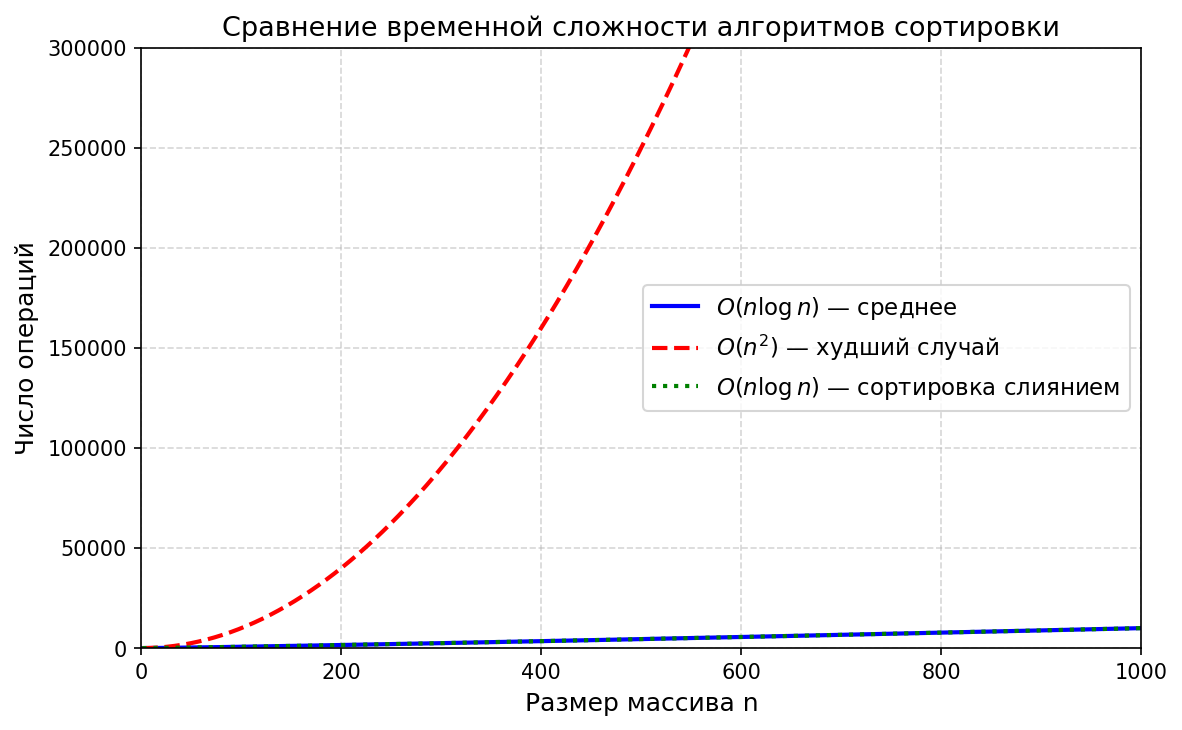
\includegraphics[width=0.85\textwidth]{images/complexity.png}
    \caption{Сравнение временной сложности алгоритмов сортировки}
    \label{fig:complexity}
\end{figure}

Как видно из рисунка~\ref{fig:complexity}, при небольших значениях \texttt{n}
разница незначительна, однако с ростом размера массива $O(n^2)$ резко
превосходит $O(n \log n)$.
